% The Analytics Edge Data Competition 2026 -- Team 3 report
% Compile: pdflatex (MiKTeX). Two passes for references.
\documentclass[11pt]{article}
\usepackage[a4paper,margin=2.2cm]{geometry}
\usepackage[T1]{fontenc}
\usepackage{lmodern}
\usepackage{microtype}
\usepackage{booktabs}
\usepackage{amsmath}
\usepackage{graphicx}
\usepackage{xcolor}
\definecolor{acc}{RGB}{31,71,136}
\definecolor{accB}{RGB}{40,105,95}
\definecolor{meas}{RGB}{176,124,34}
\usepackage{tikz}
\usetikzlibrary{positioning,arrows.meta,fit,calc,backgrounds}
\usepackage{pgfplots}
\pgfplotsset{compat=1.17}
\usepackage{caption}
\captionsetup{font=small,labelfont=bf,skip=4pt}
\usepackage{titlesec}
\titlespacing*{\section}{0pt}{7.5pt}{3.5pt}
\titlespacing*{\subsection}{0pt}{5.5pt}{2.5pt}
\titleformat{\section}{\large\bfseries\color{acc}}{\thesection}{0.6em}{}
\titleformat{\subsection}{\normalsize\bfseries}{\thesubsection}{0.6em}{}
\usepackage{fancyhdr}
\pagestyle{fancy}
\fancyhf{}
\fancyhead[L]{\small\scshape 40.016 The Analytics Edge}
\fancyhead[R]{\small\scshape Team 3}
\fancyfoot[C]{\small\thepage}
\renewcommand{\headrulewidth}{0.3pt}
\usepackage[colorlinks=true,linkcolor=acc,urlcolor=acc,citecolor=acc]{hyperref}
\setlength{\parskip}{2pt}
\setlength{\parindent}{12pt}
\widowpenalty=10000
\clubpenalty=10000

\begin{document}

% ---------------------------------------------------------------- cover page
\begin{titlepage}
\noindent
\begin{minipage}[b]{0.45\textwidth}

\includegraphics[width=40mm]{sutd_logo.pdf}
\end{minipage}%
\hfill
\begin{minipage}[b]{0.5\textwidth}
\raggedleft
{\bfseries 40.016 The Analytics Edge}\\[1mm]
Data Competition 2026
\end{minipage}

\vspace{5mm}
\noindent{\color{acc}\rule{\textwidth}{1.6pt}}

\vspace{26mm}
\noindent{\Huge\bfseries\color{acc} Predicting Choice Among\\[3.5mm] Car Safety Bundles\par}
\vspace{7mm}
\noindent{\Large Final Report \,\textperiodcentered\, Team 3 R-izzlers\par}

\vspace{16mm}
\noindent\colorbox{acc!8}{%
\begin{minipage}{\dimexpr\textwidth-2\fboxsep}
\vspace{3.5mm}
\centering
\begin{tabular}{c@{\hspace{16mm}}c}
{\large\bfseries 1.185} & {\large\bfseries 1.185}\\[0.5mm]
public leaderboard, 3rd place & private leaderboard, 4th place\\
\end{tabular}
\vspace{3.5mm}
\end{minipage}}

\vspace{20mm}
\noindent
\begin{minipage}[t]{0.48\textwidth}
{\bfseries Prepared by}\\[2.5mm]
\begin{tabular}{@{}l@{\hspace{7mm}}l}
Chia Zhi Feng & 1009327\\[0.8mm]
Kavya Santosh Nair & 1009736\\[0.8mm]
Sheil Ketan Mistry & 1009394\\[0.8mm]
Nicole Ann Chia & 1009029\\
\end{tabular}
\end{minipage}%
\hfill
\begin{minipage}[t]{0.44\textwidth}
\raggedleft
{\bfseries Course Instructors}\\[2.5mm]
Karthik Natarajan\\[0.8mm]
Yihan Du
\end{minipage}

\vfill
\noindent{\color{acc!60}\rule{\textwidth}{0.5pt}}\\[2.5mm]
\noindent Kaggle team name: \texttt{sheil\_mistry\_team\_3}\hfill Submitted: 10 August 2026
\end{titlepage}

\pagenumbering{arabic}

% ------------------------------------------------------------------- body
\section{Introduction}\label{sec:data}

Each of 1{,}135 survey respondents faced 19 choice tasks. A task shows three configured
safety bundles and a fourth option, ``none of these'', and the respondent picks one. We
predict the four choice probabilities for every task of 263 \emph{new} respondents
(4{,}997 tasks), scored by mean multiclass log loss.

Three characteristics of the data shaped our modelling decisions. First, Ch4 is the most
frequently chosen alternative, accounting for 30.2\% of training choices. Second, the 19
product attributes are ordinal tiers, so treating their levels as numerical imposes a
linearity the data does not support. Third, the test population differs materially from
training: median income rises from \$60k to \$80k (mean \$75k to \$151k), while luxury
vehicles account for 69\% of test tasks versus 9\% in training. Transfer to unseen
respondents was therefore an important part of the problem.

Our final submission combines two modelling tracks using an
equal-weight geometric pool. It achieved a log-loss of 1.185 on both the public and
private leaderboards, ranking 3rd and 4th respectively.

\section{Validation strategy}\label{sec:valid}

\noindent\textbf{Grouped folds}\par
All cross-validation was grouped by respondent. Track A and the main model-comparison
experiments used one fixed five-fold partition, while Track B used a respondent-grouped partition. Because each respondent answers 19 tasks,
row-wise splitting would allow information about the same person to appear in both
training and validation. We therefore held out complete respondents, matching the
cold-start structure of the test set.

A model's score on these respondents is its out-of-fold (OOF) log loss. Blend weights are
refit five times, each time excluding the fold being scored; we refer to scores produced
under this procedure as \emph{nested}.

\smallskip
\noindent\textbf{Estimating model variation}\par
We measured score variation across random seeds before interpreting small gains.
Improvements below this variation were treated cautiously in later model comparisons.

\begin{center}\small
\begin{tabular}{lll}
\toprule
comparison & yardstick & measured \\
\midrule
two single models & seed sd of one model & 0.00283 \\
two blends & seed sd of the blend & 0.00048 \\
one model across folds & fold-to-fold sd & 0.013 \\
\bottomrule
\end{tabular}
\end{center}

\noindent Model comparisons also use paired tests with respondent-clustered standard
errors so that differences are assessed on identical held-out rows.

\section{Final model}\label{sec:model}

The final submission combines two modelling tracks using an
equal-weight geometric pool. Track A combines listwise XGBoost with a latent-class choice
model, while Track B combines latent taste features with tree and neural utility models.
Figure~\ref{fig:arch} summarises the prediction pipeline.

\begin{figure}[t]
\centering
\resizebox{\textwidth}{!}{%
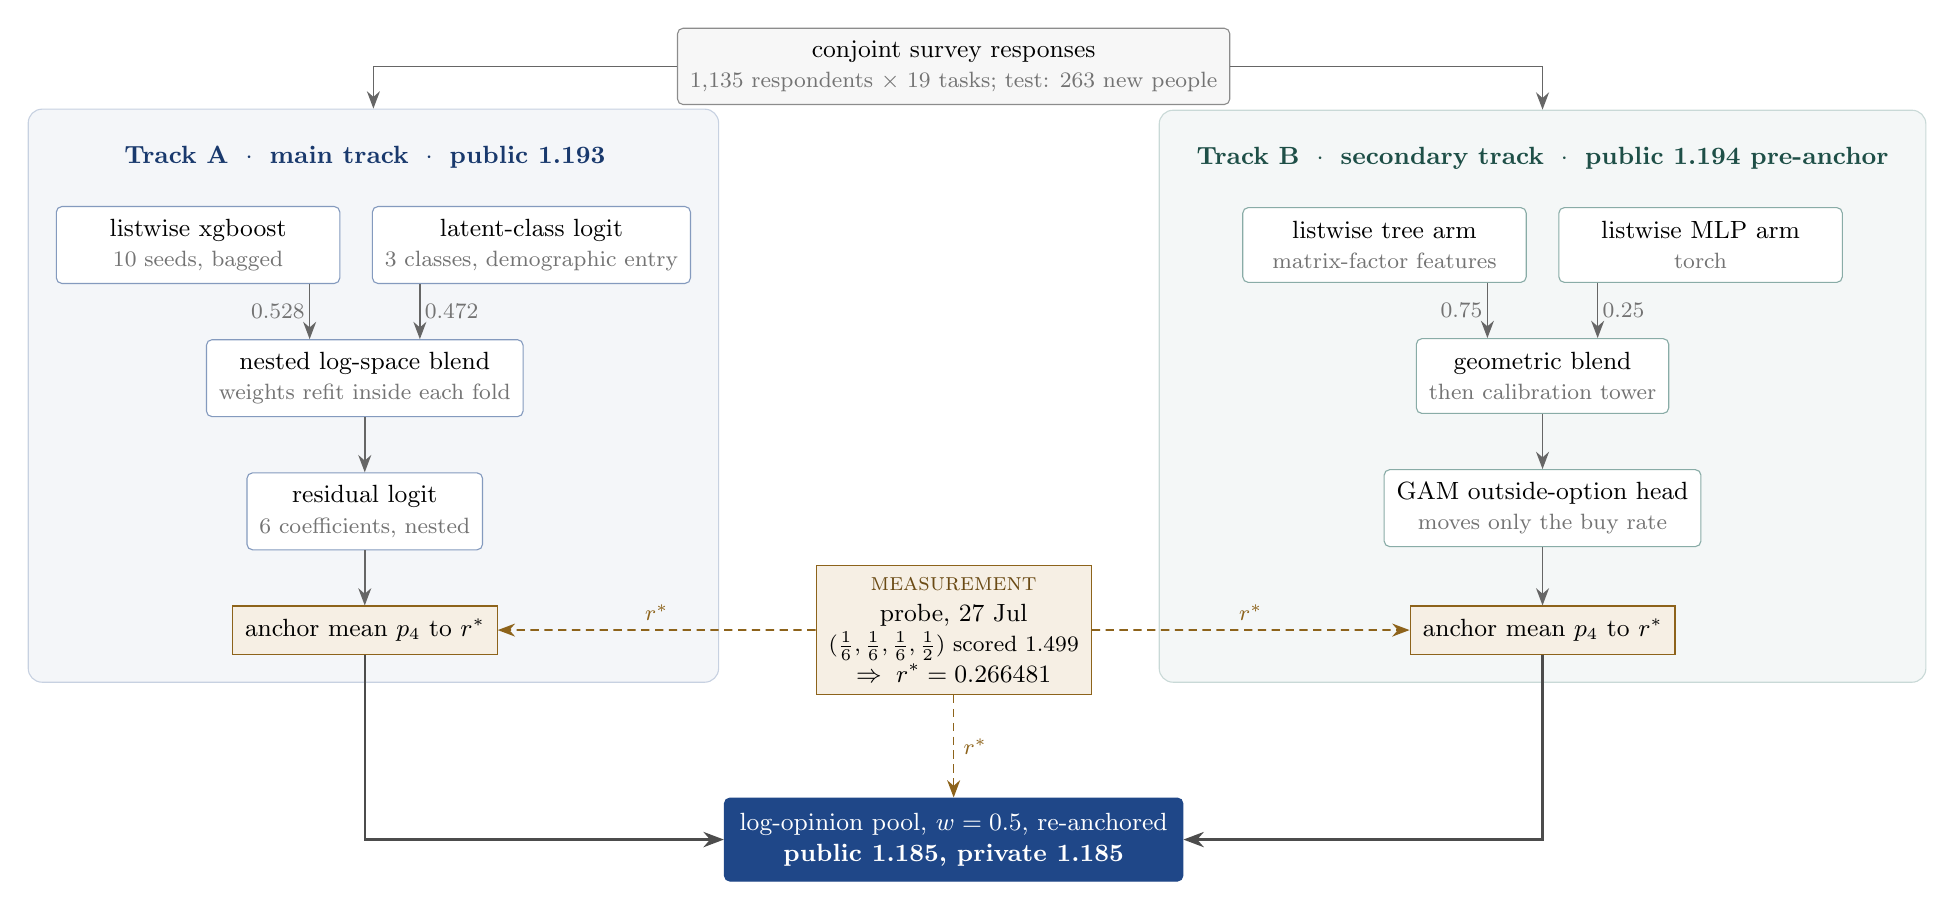
\begin{tikzpicture}[
  font=\small,
  det/.style={font=\footnotesize, text=black!55},
  box/.style={draw, rounded corners=2pt, align=center, inner sep=4.5pt, minimum height=9.5mm, fill=white},
  membA/.style={box, draw=acc!55},
  membB/.style={box, draw=accB!55},
  measbox/.style={draw=meas!80!black, fill=meas!12, align=center, inner sep=4.5pt},
  final/.style={draw=acc, fill=acc, text=white, rounded corners=2pt, align=center, inner sep=5.5pt},
  lane/.style={rounded corners=5pt, inner sep=3.5mm},
  arr/.style={-{Stealth[length=2.2mm]}, semithick, black!60},
  mainarr/.style={-{Stealth[length=2.6mm]}, thick, black!70},
  marr/.style={-{Stealth[length=2.2mm]}, semithick, densely dashed, meas!80!black},
  wlab/.style={font=\footnotesize, text=black!55, inner sep=1.5pt},
  node distance=7mm and 5mm]
\node[membA, minimum width=36mm] (xgb) {listwise xgboost\\{\footnotesize\color{black!55}10 seeds, bagged}};
\node[membA, minimum width=36mm, right=4mm of xgb] (lc) {latent-class logit\\{\footnotesize\color{black!55}3 classes, demographic entry}};
\node[membA, below=of $(xgb.south)!0.5!(lc.south)$] (blend) {nested log-space blend\\{\footnotesize\color{black!55}weights refit inside each fold}};
\node[membA, below=of blend] (rl) {residual logit\\{\footnotesize\color{black!55}6 coefficients, nested}};
\node[measbox, below=of rl] (ancA) {anchor mean $p_4$ to $r^{*}$};
\node[membB, minimum width=36mm, right=70mm of lc] (tree) {listwise tree arm\\{\footnotesize\color{black!55}matrix-factor features}};
\node[membB, minimum width=36mm, right=4mm of tree] (nn) {listwise MLP arm\\{\footnotesize\color{black!55}torch}};
\node[membB, below=of $(tree.south)!0.5!(nn.south)$] (gblend) {geometric blend\\{\footnotesize\color{black!55}then calibration tower}};
\node[membB, below=of gblend] (gam) {GAM outside-option head\\{\footnotesize\color{black!55}moves only the buy rate}};
\node[measbox] (ancB) at (gam |- ancA) {anchor mean $p_4$ to $r^{*}$};
\node[font=\small\bfseries, text=acc!80!black, anchor=south,
      above=3.5mm of $(xgb.north)!0.5!(lc.north)$] (labA) {Track A \(\;\cdot\;\) main track \(\;\cdot\;\) public 1.193};
\node[font=\small\bfseries, text=accB!75!black, anchor=south,
      above=3.5mm of $(tree.north)!0.5!(nn.north)$] (labB) {Track B \(\;\cdot\;\) secondary track \(\;\cdot\;\) public 1.194 pre-anchor};
\begin{scope}[on background layer]
\node[lane, fill=acc!5, draw=acc!25, fit=(labA)(xgb)(lc)(blend)(rl)(ancA)] (laneA) {};
\node[lane, fill=accB!5, draw=accB!25, fit=(labB)(tree)(nn)(gblend)(gam)(ancB)] (laneB) {};
\end{scope}
\node[box, draw=black!45, fill=black!3] at ($(labA.north)!0.5!(labB.north)+(0,9mm)$) (data)
  {conjoint survey responses\\{\footnotesize\color{black!55}1{,}135 respondents $\times$ 19 tasks; test: 263 new people}};
\node[measbox] at ($(ancA.east)!0.5!(ancB.west)$) (probe)
  {{\scshape\color{meas!60!black} measurement}\\probe, 27 Jul\\{\footnotesize $(\tfrac16,\tfrac16,\tfrac16,\tfrac12)$ scored 1.499}\\$\Rightarrow\; r^{*}=0.266481$};
\node[final, below=13mm of probe] (pool)
  {log-opinion pool, $w=0.5$, re-anchored\\\bfseries public 1.185, private 1.185};
\draw[arr] (data.west) -| (laneA.north);
\draw[arr] (data.east) -| (laneB.north);
\coordinate (bL) at ($(blend.north)+(-7mm,0)$);
\coordinate (bR) at ($(blend.north)+(7mm,0)$);
\coordinate (gL) at ($(gblend.north)+(-7mm,0)$);
\coordinate (gR) at ($(gblend.north)+(7mm,0)$);
\draw[arr] (bL |- xgb.south) -- node[wlab, left]{0.528} (bL);
\draw[arr] (bR |- lc.south) -- node[wlab, right]{0.472} (bR);
\draw[arr] (blend) -- (rl);
\draw[arr] (rl) -- (ancA);
\draw[arr] (gL |- tree.south) -- node[wlab, left]{0.75} (gL);
\draw[arr] (gR |- nn.south) -- node[wlab, right]{0.25} (gR);
\draw[arr] (gblend) -- (gam);
\draw[arr] (gam) -- (ancB);
\draw[mainarr] (ancA.south) |- (pool.west);
\draw[mainarr] (ancB.south) |- (pool.east);
\draw[marr] (probe.west) -- node[above, font=\footnotesize]{$r^{*}$} (ancA.east);
\draw[marr] (probe.east) -- node[above, font=\footnotesize]{$r^{*}$} (ancB.west);
\draw[marr] (probe.south) -- node[right, font=\footnotesize]{$r^{*}$} (pool.north);
\end{tikzpicture}}
\caption{The graded submission, data to file. Rounded boxes are fitted models; square
amber boxes are the one measured constant and the places it is applied; numbers on edges
are blend weights. The pool step fits nothing: $w=0.5$ was fixed before upload and never
tuned. Track A as drawn scored public 1.193; track B's public 1.194 predates its anchor
step, which was added at pooling (Section~\ref{sec:probe}).}
\label{fig:arch}
\end{figure}

\subsection{Track A: XGBoost and latent-class choice model}

Track A was built around three modelling decisions.

\emph{Part-worth coding.} Allowing each attribute level to have its own utility improved
OOF log-loss by approximately 0.020 ($z=11.8$), the largest individual modelling gain we
observed. The fitted price response falls sharply at first and then flattens
(Figure~\ref{fig:price}), which linear coding cannot represent.

\emph{Listwise utility modelling.} Representing each task as four competing alternatives
improved OOF log-loss by approximately 0.006 ($z=4.3$). XGBoost was therefore trained
using a custom choice-set objective based on the within-task softmax.

\emph{Latent preference heterogeneity.} A three-class latent-class conditional logit
improved OOF log-loss by approximately 0.013 ($z=3.8$). Class membership is predicted
from demographics only, allowing heterogeneity to be projected to unseen respondents.

The two members, a ten-seed listwise XGBoost model and the latent-class model with
task-position terms, are pooled in log space with weights 0.528 and 0.472. Their original
nested estimate was 1.12819; a later encoding audit showed that this was inflated by
roughly 0.008, giving a leak-free nested figure close to 1.136
(Section~\ref{sec:fail}).

A six-coefficient residual logit was then applied to systematic probability errors using
relative price, an outside-option constant, bundle richness relative to the best rival,
and interactions with luxury segment. This was the only late-stage residual correction
that improved both the production folds and an independent fold structure: $+0.00300$ on
the former and $+0.00628$ on the latter. The combined evidence was still modest, so we
treated the correction as a small refinement rather than a major source of performance.

\subsection{Track B: taste features with tree and neural models}

Track B was developed as a second route to the four-choice probability
distribution.

Repeated choices were first converted into respondent-level preference profiles. For each task, the selected alternative was compared with those actually offered, so
the profile captured relative responses to price, safety attributes and the outside option.
Aggregating these signals over 19 tasks produced a respondent-by-preference matrix.

A rank-3 matrix factorisation compressed this matrix into three latent taste coordinates.
Because test respondents have no observed choice history, these coordinates could not be
computed directly at prediction time. We therefore fitted demographic mappings from the
observed respondent variables to the three latent coordinates and used them to project
unseen respondents into the same taste space. The projected taste variables were then
converted into alternative-level compatibility features for the predictive models.

The matrix-factorisation stage does not itself produce the final choice probabilities.
Instead, Track B uses two four-choice utility learners: a listwise XGBoost model and a
Torch multilayer perceptron. Their predictions are combined geometrically, with
approximately 75\% weight on XGBoost and 25\% on the neural model.

A small probability-calibration stage follows. Segment-level and low-dimensional residual
corrections are applied first, after which a binomial GAM supplies an additional estimate
of Ch4 propensity. The GAM estimate is mixed into the existing Ch4 probability at 25\%.
The remaining probability mass is redistributed proportionally across Ch1--Ch3, so the
relative ranking of the three purchase bundles from the primary tree--neural model is
preserved.

Track B scored 1.194 publicly before the final Ch4 calibration. Its blended arms score
1.153 OOF on its own respondent-grouped partition. Its value in the final ensemble was therefore complementarity rather than superior
standalone performance.

\subsection{Aggregate Ch4 calibration}\label{sec:probe}

On 27 July, we used one submission as a diagnostic rather than as a candidate model. The
file \texttt{probe\_alt4.csv} predicts
$(\tfrac16,\tfrac16,\tfrac16,\tfrac12)$ on every row. For a constant prediction,
\[
L=(1-r)\log 6+r\log 2
\qquad\Longrightarrow\qquad
r^{*}=\frac{\log 6-1.499}{\log 3}=0.266481.
\]

The returned public score therefore implied a Ch4 share of approximately 0.2665 on the
public leaderboard subset. We treated this as a competition-stage calibration target
rather than as a parameter estimated from training data.

Both tracks were adjusted so that their mean predicted Ch4 probability matched
$r^{*}$, while preserving the relative probabilities of Ch1--Ch3. This adjustment had
little effect on Track A but materially improved Track B, whose mean Ch4 probability had
previously been 0.211.

\subsection{Final two-track ensemble}\label{sub:pool}

The two tracks had similar standalone public performance but were produced through
different modelling pipelines. Rather than introduce another late-stage tuned parameter,
we fixed the final ensemble weight at $w=0.5$.

Geometric pooling also provides a useful safety property. If the pooled probabilities are
formed as $P_k \propto A_k^{1-w}B_k^w$, H\"older's inequality implies that, on a fixed
evaluation set,
\[
\mathrm{loss(pool)} \le (1-w)L_A+wL_B \le \max(L_A,L_B).
\]
This supported combining the tracks without a finely tuned ensemble weight.

The tracks were also meaningfully different in practice. Their within-purchase
probabilities differed by 0.0129 on average, compared with a 0.0055 difference obtained
from simply reseeding one model, and their predicted probability vectors differed on
96.6\% of rows. This supported treating the two tracks as complementary ensemble members
rather than minor variants of the same learner.

\subsection{Alternative models considered}\label{sub:field}

Before Track A's two blend members were chosen, nine model families were fitted under the
same respondent-grouped validation framework. This comparison was useful because it
separated improvements from additional model capacity from improvements that better
matched the structure of the choice problem.

\begin{center}\small
\begin{tabular}{lrl}
\toprule
model family & OOF & verdict \\
\midrule
listwise xgboost, 10-seed bag & 1.13682 & \textbf{blend member 1} \\
latent-class logit, 3 classes & 1.13863 & \textbf{blend member 2} \\
nested logit, \{bundles\} vs \{none\} & 1.15681 & no gain over plain logit \\
part-worth conditional logit & 1.15686 & one-class special case \\
elastic-net logit & 1.16718 & shrinkage cannot replace part-worths \\
two-stage buy / bundle model & 1.17169 & splits one utility scale in two \\
mixed logit & 1.17281 & predicts a population average \\
wide four-class xgboost & 1.17456 & cannot compare within a choice set \\
hierarchical Bayes & 1.23703 & cold-start limitation \\
\midrule
nested blend & 1.12819 & honest $\approx 1.136$ (Section~\ref{sec:fail}) \\
\bottomrule
\end{tabular}
\end{center}

\noindent The comparison suggests that the strongest gains came from modelling the
choice-set structure directly, allowing nonlinear part-worths, and representing
heterogeneity in a way that could still be estimated for unseen respondents. More
flexible models were not automatically better under the cold-start evaluation.

\section{Model development and rejected experiments}\label{sec:fail}

Several rejected experiments materially changed how we evaluated later modelling
decisions.

\subsection{Seed variation and apparent gains}

Refitting the same XGBoost configuration under ten seeds moved OOF log-loss across a
range of 0.0090 (sd 0.00283). This invalidated one apparent gain from a monotone price
constraint: an initial improvement of $+0.00172$ became $-0.00034$ under a paired
ten-seed comparison, with 95\% CI $[-0.00159,+0.00092]$. The constrained variant was
therefore removed.

Averaging predetermined seeds reduced Monte-Carlo variation without introducing another
validation-selected hyperparameter.

\subsection{Leakage despite respondent-grouped folds}

One derived residual feature produced an unusually large apparent improvement of about
0.03. Although respondent folds were separated correctly, an upstream baseline prediction
had indirectly used information from the scored fold. Rebuilding the feature while
excluding both the reference and evaluation folds removed the gain
($-0.00430$, $z=-4.54$).

A second issue affected a design-share encoding constructed before the CV loop. Because
the encoding was generated once and then reused inside cross-validation, training rows
could contain summaries influenced by the scored fold even though the respondent split
itself was correct. The feature initially appeared to improve OOF loss by about 0.022 and
remained in the production pipeline for many iterations.

Three checks eventually exposed the problem. First, an honestly reconstructed version
produced a negative value of $-0.00596$ ($z=-3.53$). Second, the apparent gain increased
with tree depth, from approximately $-0.0004$ at depth 4 to $+0.078$ at depth 10, which is
more consistent with a flexible model exploiting leakage than with a stable predictive
effect. Third, removing the feature changed the ranking of the earlier hyperparameter
sweep. These cases showed that grouped folds alone are insufficient if feature
construction itself uses information from the evaluation fold.

\subsection{How this changed our validation process}

After the leakage audit, small improvements in the original OOF metric were treated
cautiously. A segment-reweighted OOF score was used as a secondary diagnostic because it
tracked the public leaderboard more closely when leak-free, but its effective sample of
208 respondents made it unsuitable as a training objective.

\section{Model insights}\label{sec:insight}

\begin{figure}[b]
\centering
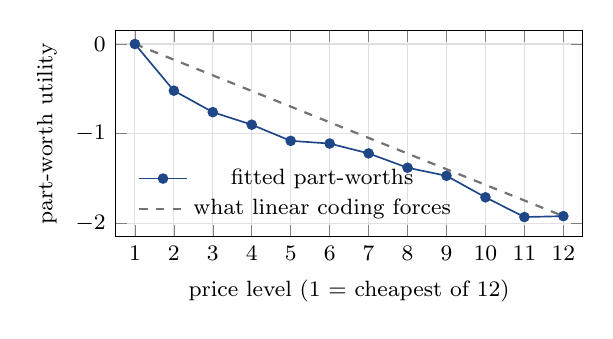
\begin{tikzpicture}
\begin{axis}[
  width=0.62\textwidth, height=4.2cm,
  xlabel={price level (1 = cheapest of 12)}, ylabel={part-worth utility},
  xmin=0.5, xmax=12.5, ymin=-2.15, ymax=0.15,
  xtick={1,...,12}, tick label style={font=\footnotesize},
  label style={font=\footnotesize},
  grid=major, grid style={black!12},
  legend style={font=\footnotesize, at={(0.03,0.03)}, anchor=south west, draw=none, fill=none}]
\addplot[color=acc, mark=*, mark size=1.6pt, semithick] coordinates
{(1,0) (2,-0.52) (3,-0.76) (4,-0.90) (5,-1.08) (6,-1.11) (7,-1.22) (8,-1.38) (9,-1.47) (10,-1.71) (11,-1.93) (12,-1.92)};
\addlegendentry{fitted part-worths}
\addplot[color=black!55, dashed, thick] coordinates {(1,0) (12,-1.92)};
\addlegendentry{what linear coding forces}
\end{axis}
\end{tikzpicture}
\caption{Price response flattens: the first step up from the cheapest level costs 0.52
utility, later steps average 0.13, and the top two levels are nearly identical. Freeing
this shape was worth $+0.020$ log loss.}
\label{fig:price}
\end{figure}

\subsection{Latent preference groups and price response}

The latent-class model splits respondents into three near-equal segments. Membership is
predicted from demographics, with annual mileage, night driving, education and parking
situation among the strongest drivers:

\begin{center}\small
\begin{tabular}{lccc}
\toprule
segment & share & price response & outside-option constant \\
\midrule
price-sensitive group & 36.6\% & $-1.65$, steady decline & $-1.40$ \\
weakly price-sensitive / premium-oriented group & 32.1\% & $+0.50$, flat to positive & $-1.30$ \\
opt-out-prone group & 31.4\% & $-0.60$, mild & $+0.17$ \\
\bottomrule
\end{tabular}
\end{center}

The aggregate price curve flattens at higher price levels, but the latent classes suggest
that part of this shape comes from mixing respondents with different price sensitivities.
The first group shows a steep and consistently negative price response, while the second
is close to flat over much of the range and the third is comparatively mild. Averaging
these curves naturally produces a flatter aggregate response even when no single segment
has exactly that shape.

The positive price response in the second class may reflect premium orientation or
residual confounding between price and bundle richness, so it should not be interpreted
causally. The third class is notable for its higher baseline tendency to choose Ch4.
Commercially, this suggests that price changes alone are unlikely to affect every
respondent group equally.

\subsection{Discrete heterogeneity transferred better under cold start}

Mixed logit estimated substantial heterogeneity but scored 1.173, while hierarchical
Bayes scored 1.23703 overall. The cold-start problem is visible when the same HB model is
scored using respondent-specific fitted tastes versus population-average tastes:

\begin{center}\small
\begin{tabular}{lc}
\toprule
prediction for the same rows & log loss \\
\midrule
each respondent's own fitted tastes & 0.352 \\
population-averaged tastes & 1.229 \\
\bottomrule
\end{tabular}
\end{center}

The 0.877 difference shows how much respondent-specific information becomes unavailable
for unseen test respondents. Hierarchical Bayes is powerful when a respondent's own
choice history is available, but much of that advantage disappears when predicting for a
new person.

The latent-class model transferred better because it routes heterogeneity through a much
lower-dimensional structure that can be estimated from demographics available at
prediction time. Removing demographics improved HB from 1.237 to 1.164, while the same
information accounted for 93\% of the latent-class gain. This does not mean continuous
heterogeneity is inherently unsuitable; here, the discrete representation provided a
better bias--variance trade-off under cold start.

\subsection{Separating opt-out did not improve predictive fit}

A two-stage model that first predicted buy/no-buy and then bundle choice scored 1.172, and
a nested-logit treatment of the outside option matched plain multinomial logit to three
decimals. For this dataset, the unified utility specification was therefore sufficient.

\subsection{Task position and changing price sensitivity}\label{sub:fatigue}

\begin{figure}[b]
\centering
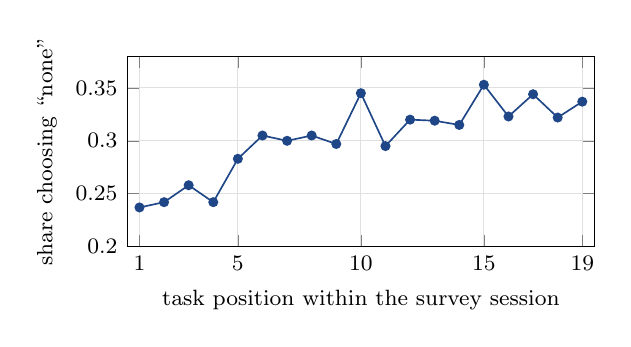
\begin{tikzpicture}
\begin{axis}[
  width=0.62\textwidth, height=4.0cm,
  xlabel={task position within the survey session}, ylabel={share choosing ``none''},
  xmin=0.5, xmax=19.5, ymin=0.20, ymax=0.38,
  xtick={1,5,10,15,19}, ytick={0.20,0.25,0.30,0.35},
  yticklabel={\pgfmathprintnumber{\tick}},
  tick label style={font=\footnotesize},
  label style={font=\footnotesize},
  grid=major, grid style={black!12}]
\addplot[color=acc, mark=*, mark size=1.5pt, semithick] coordinates
{(1,0.237) (2,0.242) (3,0.258) (4,0.242) (5,0.283) (6,0.305) (7,0.300) (8,0.305)
 (9,0.297) (10,0.345) (11,0.295) (12,0.320) (13,0.319) (14,0.315) (15,0.353)
 (16,0.323) (17,0.344) (18,0.322) (19,0.337)};
\end{axis}
\end{tikzpicture}
\caption{Raw training data: the share choosing ``none'' rises from 23.7\% on the first
task to above 33\% late in the session.}
\label{fig:fatigue}
\end{figure}

The walk-away rate rises across the 19 tasks of a survey session
(Figure~\ref{fig:fatigue}). Adding task-position terms to the latent-class model improved
OOF log-loss by $+0.0053$ ($z=6.3$) and replicated on an independent fold structure
($+0.0042$, $z=4.7$). We also compared this explanation with a pure scale-drift
specification in which later
answers simply become noisier. The changing-price-sensitivity specification reproduced
essentially all of the observed increase in Ch4, whereas scale drift reproduced very
little. The fitted interaction therefore suggests that later responses are associated
with stronger price sensitivity rather than simply greater response noise.

\subsection{Population shift and transfer to the test set}

The latent-class model predicted a lower Ch4 rate for the wealthier test population
(0.223 versus 0.302 in training). The public diagnostic implied 0.266, confirming the
direction but showing that the model overstated the magnitude. We also checked whether
the main modelling gains survived reweighting toward the test income distribution:
part-worth coding retained about 101\% of its value, the listwise objective 112\%, and
the latent-class model 79\%. This suggested that the first two improvements transferred
well, while the heterogeneity model was more sensitive to population composition. The
gap between the model-implied Ch4 rate and the public diagnostic motivated the final
aggregate Ch4 calibration.

\subsection{Remaining sources of prediction error}

An oracle using each respondent's own observed choice rates scores 0.986 against 1.130 for
the blend as it stood when measured, leaving a substantial gap associated with
person-specific behaviour. A variance decomposition shows that Ch4 is much more personal
than the three bundle choices: roughly 33\% of its variation is between respondents,
compared with about 5--7\% for the bundles.

Demographics explain only 11.2\% of that between-respondent variation in Ch4. In other
words, most of the stable individual tendency to opt out is not recoverable from the
variables supplied in the competition. This places a practical limit on the amount of
respondent-specific variation that any model using the available features can recover.

\section{Public and private leaderboard performance}\label{sec:lb}

\subsection{Local validation versus leaderboard performance}

\begin{center}\small
\begin{tabular}{cccc}
\toprule
local nested OOF & public & offset & transfer of local gain \\
\midrule
1.17683 & 1.223 & $+0.046$ & first submission \\
1.13878 & 1.201 & $+0.062$ & $\sim$58\% \\
1.13556 & 1.201 & $+0.065$ & not visible \\
1.13044 & 1.199 & $+0.069$ & $\sim$24--39\% \\
\bottomrule
\end{tabular}
\end{center}

Local OOF scores were consistently lower than public leaderboard loss by approximately
0.05--0.07, reflecting both population differences and accumulated model-selection
optimism. Transfer of small local gains weakened over time, so the leaderboard was used
mainly for limited aggregate diagnostics rather than repeated fine-grained model
selection.

\subsection{Pre-upload score forecasts}

We recorded score forecasts before the corresponding submissions were evaluated, giving
a prospective check on the validation and calibration logic.

\begin{center}\small
\begin{tabular}{lccc}
\toprule
quantity & forecast & band & returned \\
\midrule
Track A final file & 1.1930 & point forecast & 1.193 \\
graded pool & 1.186 & 1.184--1.189 & \textbf{1.185} \\
\bottomrule
\end{tabular}
\end{center}

\subsection{Private leaderboard results}

The final private score was also 1.185, showing no detectable deterioration at the
leaderboard's displayed precision. This is consistent with the conservative final
ensemble and with the fact that the aggregate Ch4 calibration, estimated only from the
public subset, did not produce an observable loss increase on the private rows.

The rank moved from 3rd to 4th despite the unchanged score. Because all teams are scored
on the same private rows, rank differences depend on where models disagree rather than on
the absolute sampling variability of one team's score alone. We therefore interpret the
unchanged loss as evidence of stable transfer, while treating the one-place rank change as
compatible with ordinary paired ranking variation.

\section{Limitations}\label{sec:limits}

A substantial amount of respondent-level variation remains unexplained by the available
variables. Some gains may not transfer directly to a different experimental design or
population, particularly those routed through choice-set identity and latent-class
membership. Evidence for preference heterogeneity was consistent, but the exact class
boundaries were less stable: several nearby class specifications fit similarly, so the
three segments should be treated as a useful predictive summary rather than as uniquely
identified consumer types.

The submitted tree pipeline still contains the design-share feature discussed in
Section~\ref{sec:fail}. Subsequent ablation suggested that removing it was approximately
leaderboard-neutral, but we did not rebuild the final candidate late in the submission
window. We would exclude this feature in a future implementation.

Finally, we optimise average log loss only; no subgroup is separately calibrated, and
predictions are least reliable where support is thinnest, particularly the wealthy luxury
segments concentrated in the test set.

\section{Reproducibility}\label{sec:repro}

Fresh training approximately reconstructs both modelling procedures. Track A can be
rerun from its modelling script followed by the residual-logit and calibration steps,
while Track B has its own end-to-end runner. Multithreaded XGBoost and Torch may produce
small numerical differences across machines, so fresh retraining is not expected to be
bit-identical.

Separately, a deterministic reconstruction using \texttt{build\_candidates.R}, the
pinned Track A and Track B outputs, and the Ch4 calibration agrees with the scored
submission to within $1.1\times10^{-15}$. Two implementation details are documented because
they affected reproduction: XGBoost 3.x returns a matrix from \texttt{predict} where
older versions returned a vector, and conditional-logit designs must place reference
levels carefully because variables constant within a choice set are unidentified.

\section{Conclusion}\label{sec:conc}

Three modelling choices made early in the project---part-worth coding, a listwise
objective, and demographically routed discrete heterogeneity---accounted for most of the
predictive performance we achieved. Later work contributed mainly by clarifying where the
remaining error lies, identifying two sources of leakage, and improving how we interpreted
small validation gains.

The final submission used a fixed two-track ensemble and achieved a log-loss of 1.185 on
both the public and private subsets. Three lessons were most useful in retrospect:
estimate stochastic variation before acting on small gains, construct leak-free comparisons
for features that appear unusually strong, and validate on respondents excluded from
fitting when the test set consists of unseen respondents.

\end{document}